%! Author = 96171
%! Date = 23/05/2021

% Preamble
\documentclass[11pt]{article}
\usepackage[utf8]{inputenc}
\PassOptionsToPackage{hyphens}{url}
\usepackage[colorlinks = true,
            linkcolor = blue,
            urlcolor  = blue,
            citecolor = blue,
            anchorcolor = blue]{hyperref}
\usepackage{graphicx}
\usepackage{caption}
\usepackage{subcaption}
\usepackage[section]{placeins}
\usepackage{float}
\usepackage[utf8]{inputenc}
\usepackage{multirow}
\usepackage{csquotes}
\usepackage{xcolor}
\usepackage{amsmath}
\usepackage{longtable}
\usepackage[T1]{fontenc}
\usepackage[normalem]{ulem}
\usepackage{footmisc}
\useunder{\uline}{\ul}{}

% Packages
\usepackage{amsmath}

% Document
\begin{document}

    \section{Advanced ML Evaluation Techniques}
In this paper, authors seek to solve the problem of predicting students who are at risk of dropping out of highschool or not. They have a \textbf{binary classification problem} and they predict if the student graduates (0) or does not (1). School principals want to see if they can have enough budget to afford those - \textbf{at an early stage} - that are at risk of not graduating and help them with additional materials. Non-Machine learning practitioners do not value regular evaluation metrics like precision and recall because it means nothing to them, they want some evaluation techniques that could help understand the predictions more from their point of view

\subsection*{Disclaimer}
\begin{itemize}
\item I have read only sections 5 \& 6 from the paper as instructed by Dr. Fatima
\item I have found a github repository for their work here: \url{https://github.com/dssg/student-early-warning} but their work is not complete at all, the only thing that they did - with regards to sections 5 \& 6, is compute the \textbf{\textit{risk}}. The rest of the work is done solely by me.
\item I used the data they provided in their github repository to complete my work, they also do not provide the complete data and there are differences between the column names mentioned in the paper and the columns in the dataset they provide. But I still worked with this incomplete version of the data
\end{itemize}

\subsection{Analysis of Predictive Models}
School districts are interested in identifying those students who are are at risk of not graduating high school on time so that plan their resource allocation ahead of time.

\noindent \textbf{Goal:} predict if a student is at \textbf{risk} of not graduating high school on time

\subsection{Evaluation Using Traditional Metrics}
\begin{itemize}
\item We have a binary outcome, use standard evaluation metrics such as \textit{accuracy, precision, recall, f-measure, and AUC}
\item Their data is \textbf{imbalanced}:
\begin{enumerate}
\item \textbf{Class 0: 91.4\%}
\item \textbf{Class 1: 8.6 \%}
\end{enumerate}

\item I must do a \textbf{stratified} split of classes between training and testing such that if the original data has X\% 0s and Y\% 1s, then the training as well as the testing must also have X\% 0s and Y\%  1s

\item I have added \textbf{SMOTE} so that we can \textbf{oversample} our \textbf{training} data before predicting

\item I used MinMax Scaling (just for now because my focus is on the implementation of the ideas in sections 5 \& 6)

\item In this paper they only use shallow models, this what I also do (just for now because my focus is on the implementation of the ideas in sections 5 \& 6)

\item In Figure \ref{plots/toydata/Fig:roccurves} below, I show the ROC curves of various models
\end{itemize}

\begin{figure}[H]
\centering
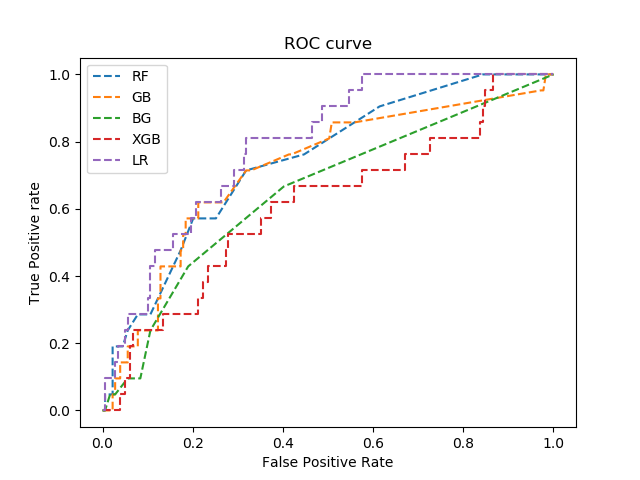
\includegraphics[scale=0.5]{plots/toydata/roccurves.png}
\caption{ROC Curves of various shallow models trained on the data provided}
\label{Fig:roccurves}
\end{figure}

\subsection{Problem with Standard Evaluation Metrics}
\begin{enumerate}
\item Educators think about the performance of an algorithm in a slightly different fashion
\item the availability of resources varies with time. For example, a school might support 100 students in 2012, and 75 in 2013.
\item We want to build algorithms that can cater to these changing settings
\end{enumerate}

\subsection{Solution: Risk Estimates}
\begin{itemize}
\item an algorithm, to cater to their needs, must provide them with a list of students ranked by some measure of \textit{risk} such that, the students at the top of the list are at a higher risk of not graduating on time.

\item Once educators have such a ranked list, they can choose the \textbf{top k} students from it and provide assistance to them

\item \textbf{Challenge:} We only have binary records, but fortunately, all classification algorithms provide internally a probability of each class we have, we can use this probability to derive our \textbf{risk} measure
\end{itemize}

\subsection{Ensuring Quality Of Risk
Estimates}
\subsubsection{From Models to Risk Estimates}
\begin{itemize}
\item The output of our predictions are binary: either 0 (will graduate on time) or 1 (will not graduate on time)
\item Algorithms allow us to get the  \textbf{probability} of each class. Here, we focus on the probability of the \textbf{positive} class (which shows the probability of not graduating on time). We use the probability of the predictions on the \textbf{final testing data }
\end{itemize}

\subsubsection{Measuring the Goodness of Risk Scores}
\begin{itemize}
\item We first get the probability of not graduating on time (class: 1) for each of the testing instances (students) we have. We call this \textbf{\textit{risk}}

\item Rank the testing instances (students) in descending order of \textbf{risk} estimates. This way, students with higher probability of not graduating on time are at the top of the list.

\item Group students into \textbf{bins (percentiles)} based on their risk scores. We can decide, for example, to choose 10 bins, and when we do, then the students who fall between the 10th and 20th percentile have very little risk scores, those between 20th and 30th have more risk scores than the latter

\item \textcolor{blue}{My problem with this is as follows: we are doing the 3 bullets above for all the algorithms we have. The distribution of risk scores, for un-balanced classification problems, is usually very skewed and therefore, we can have the following 2 scenarios:}
\begin{itemize}
\item We might not be able to group them into 10 bins for example because each bin must have the same number of instances and that might not be possible in the un-balanced skewed distribution
\item A possible solution to the problem above is to decrease the number of bins.
\item Even if we decrease the number of bins, we might not be able to attain the same number of bins for every algorithm we have. If you look at Figure 2 in their paper, you see that for all algorithms they were able to distribute risk scores into 10 bins, but in case one is not able, we cannot produce such a plot
\item One solution is to distribute them into bins but \textbf{without guaranteeing the same number of instances in each bin  }
\item Even if we are able to produce such a plot, the 10 bins won't be unique (in terms of lower and upper limits) for each algorithm. Is that valid to work with ?
\end{itemize}

\item \textcolor{blue}{SOLUTION: I fixed this problem. I enforced the same number of items to happen in each bin \textbf{according to the number of predictions}. Number of items per bin $= number of predictions // nb bins $. The $//$ in python is an \textbf{integer division} operator to divide two numbers and round their quotient down to nearest integer. This will make sure that all bins have the same number of instances (except for 1 bin if it happens that the $number of predictions$ and $nb bins$ are not divisible)}


\item For each bin, we produce the \textbf{mean empirical risk} which is the fraction of students, from that bin, who actually (as per ground truth) fail to graduate on time.
\item This curve is called \textbf{mean empirical risk} curve
\item An algorithm is considered to be producing good predictions if its empirical risk curve is \textbf{monotonically non-decreasing} (as the risk scores increase, we have more \textbf{correct} predictions about the positive class (more students who actually - as per ground truth - fail to graduate on time))
\end{itemize}

I present below the empirical risk curve of the shallow models I trained on - \textbf{with incorporating SMOTE} and MinMax Scaling
\begin{figure}[H]
\centering
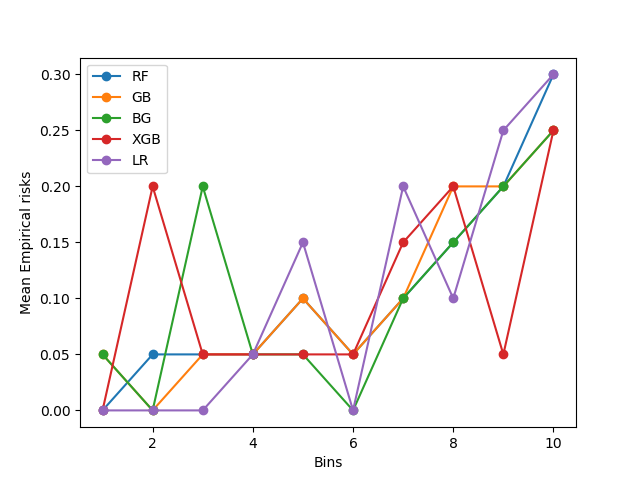
\includegraphics[scale=0.5]{plots/toydata/meanempiricalrisks.png}
\caption{Mean Empirical Risks per Model}
\label{Fig:MeanEmpiricalRisks}
\end{figure}

\subsubsection{Comparative Evaluation of Risk Estimates}
It is good to see the models performances on the \textbf{Top K} students \textbf{at risk}. The steps we do to attain this:
\begin{enumerate}
\item Rank Testing instances (students) by their \textbf{risk} scores
\item Define a list of \textbf{K}s
\item For each value \textbf{k} of \textbf{K}:
\begin{enumerate}
\item get the top \textbf{k} predicted values
\item get the ground truth  of these \textbf{top k}
\item compute the precision/recall
\end{enumerate}
\end{enumerate}
\noindent We get the precision and recall at top K and we produce the following curves:

\begin{figure}[H]
\centering
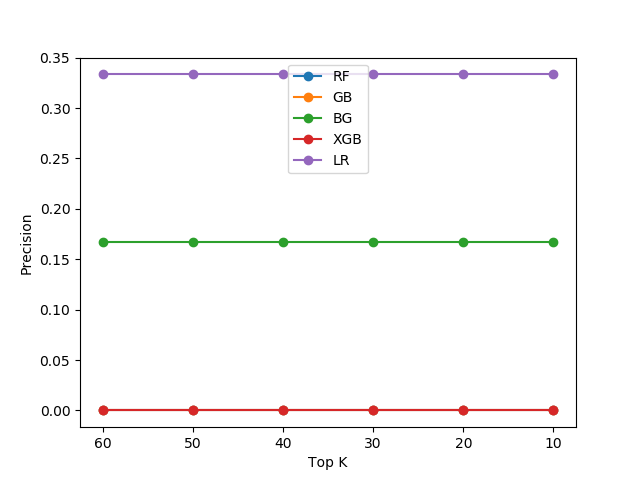
\includegraphics[scale=0.5]{plots/toydata/precisionstopK.png}
\caption{Precision at Top K}
\label{Fig:prectopk}
\end{figure}


\begin{figure}[H]
\centering
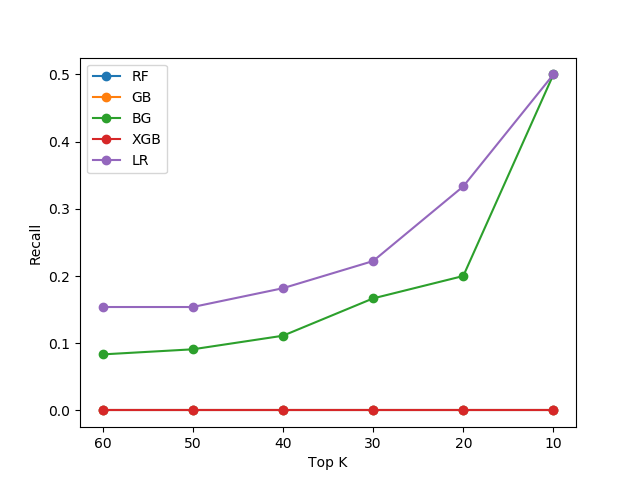
\includegraphics[scale=0.5]{plots/toydata/recallstopK.png}
\caption{Recall at Top K}
\label{Fig:prectopk}
\end{figure}

\subsection{Interpreting Classifier Outputs - FP Growth}
\subsection*{Frequent Patterns}
To understand FP Growth algorithm, we need to first understand association rules.

Association Rules uncover the relationship between two or more attributes. It is mainly in the form of- If antecedent than consequent.  For example, a supermarket sees that there are 200 customers on Friday evening. Out of the 200 customers, 100 bought chicken, and out of the 100 customers who bought chicken, 50 have bought Onions. Thus, the association rule would be- If customers buy chicken then buy onion too, with a support of 50/200 = 25\% and a confidence of 50/100=50\%.

\textbf{References:} \url{https://www.mygreatlearning.com/blog/understanding-fp-growth-algorithm/}

\subsection{Technicalities}
\noindent Usually, for identifying frequent patterns, we are represented with a \textbf{transactions} dataset, where each row represents \textbf{a set of items} bought by a customer. \textbf{However, we do not have transaction, we rather have multivariate dataset with a bunch of numerical columns. How can we do it?}

\textbf{\textcolor{blue}{Disclaimer: The methodology below presents my own solution of the problem, I am not able to find such a technique anywhere on the internet.}}

In order to \textbf{present} values as items:
\begin{enumerate}
\item Consider Each column value, in a row, as being an \textbf{item} bought by the customer.
\item Our values are numeric, therefore, to avoid redundancy, I categorize the values as follows:
\begin{itemize}
\item value $<=$ 25th percentile
\item 25th percentile $<$ value $<=$ 75th percentile
\item value $>$ 75th percentile
\end{itemize}
\item Do the categorization above, \textbf{per column}, for all values in the dataset
\item Achieve the so called "Item Dataset" where each row has one item (from the categories generated above) per column
\item Apply the FP-growth Technique on the generated "Item Dataset"
\item Extract the most frequent patterns
\end{enumerate}

The reason I did the aforementioned methodology above is because, in the \textbf{paper we are referencing (montogemery)}, they have frequent patterns like (GPA $>$ 2.0) and (Absence rate $<=$ 0.1), therefore I deduced that these can be taken by doing 'quartiles' of the distribution of values we have per column.

\subsection{Characterizing Prediction Mistakes}
\begin{enumerate}
\item Get all frequent patterns using the methodology I created above that incorporates FP-Growth
\item Rank predictions based on risk score probabilistic estimates

\item Create a new field called \textit{mistake} which is 1 if the prediction does not match ground truth and 0 otherwise

\item \textbf{For each frequent pattern} identify the \textbf{probability of mistake} by computing the number of mistakes done per frequent pattern

\item Do all of the above bullets \textbf{for each model. Therefore, we end up with a probability of mistake for each frequent pattern, per model}
\end{enumerate}



\subsection{Comparing Classifier Predictions}
When we present educators with a suite of algorithms, they are keen on understanding the differences between \textit{rank orderings} produced by each of these algorithms.

\noindent We will be using \textbf{Jaccard Similarity} for measuring similarity between predictions, \textbf{also at Top K}:

Let's say we have 200 testing instances (students). One model might put the highest risk score for the 180th testing instance, another model might put the highest risk score for the 190th testing instance. Therefore, it is important to note that in this exercise, we find which testing instances were chosen to be in the top k between model 1 and model 2, and we compute, using the jaccard similarity, the intersection of these testing instances (over their union). Good models must have very high intersections if they are classifying instances properly.

\begin{enumerate}
\item Get all possible \textbf{combinations} of model pairs (we are using a suite of models)
\item For each model pair, and for each \textbf{k} in \textbf{K}:
\begin{enumerate}
\item get the testing instances at top \textbf{k} from model 1 of the model pair
\item get the testing instances at top \textbf{k} from model 2 of the model pair
\item Compute jaccard similarity as the intersection of the two testing instances from each model over their union
\end{enumerate}
\end{enumerate}

After doing this, we get the following results:
\begin{figure}[H]
\centering
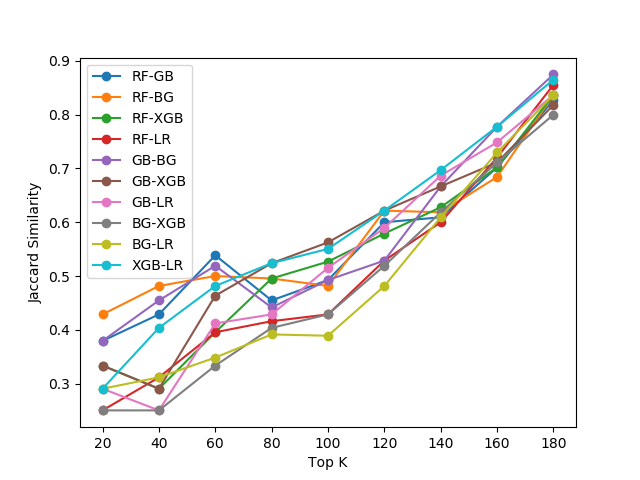
\includegraphics[scale=0.6]{plots/toydata/jaccardtopK.png}
\label{Fig:jaccardtopk}
\caption{Jaccard Similarity of students at risk for various algorithms}
\end{figure}


% \section{Advanced ML Evaluation of Fake News Experiments}
% We have already done the fake news experiments before, and for each experiment \textbf{with the exception of Expriment 2}, we have saved the \textbf{trained models}. We have made our code \textbf{accept trained models}, and assess their performance on \textbf{testing dataset} passed by the user, with the performace asssessed, hereafter, by advanced ML Evaluation techniques presented in this report.

% \subsection*{Fake News Repository}
% The fake news repository with latest experiments is found here on bitbucket in the latest folder called \textit{Hiyam}: \url{https://bitbucket.org/rba15/fake_news_detection/src/master/Hiyam/}

% \subsection{Experiment 1}
% In Experiment 1, we have trained a suit of \textbf{shallow} ML models on the FA-KES training data and tested it on the FA-KES testing data as well. Ofcourse, it is important to note that we have split the original FA-KES data in a \textbf{stratified manner}, hereafter, maintaining the same class distribution between training and testing dataset splits.

% \noindent We have chosen the \textbf{number of bins to be equal to 3}. By the number of bins, we mean the bins were the probabilistic risk scores fall in, in ascending order (smaller bins have smaller risk scores; higher bins have higher risk scores)

% \subsubsection{Mean Empirical Risks}
% \begin{figure}[H]
% 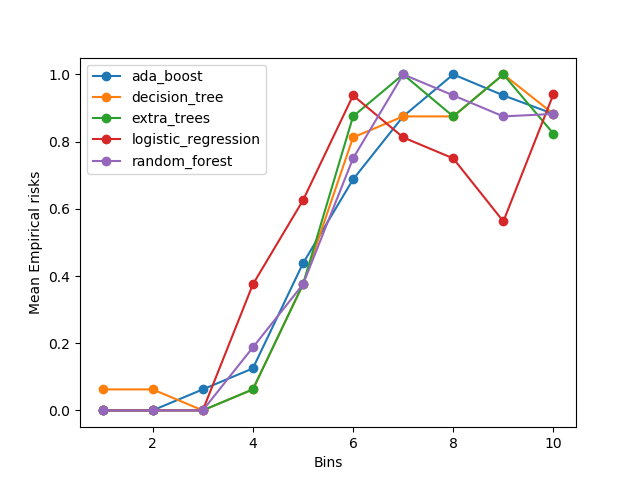
\includegraphics[scale=0.6]{plots/fakenewsexp1/meanempiricalrisks.png}
% \caption{plot that shows the mean empirical risks across the 3 bins}
% \end{figure}

% We realize that the mean empirical risks for all models is non-decreasing, indicating that our \textbf{trained models} are successful at giving higher risks to instances who are actually, \textbf{as per ground truth}, classified as being \textbf{true}

% \noindent We realize that the logistic regression model's mean empirical risk curve decreases when the number of bins is 9.

% \noindent In general, several models have their mean empirical risk decrease for a high bin number, suggesting that the models at extreme cases were the instances classified as being \textbf{true} do not assign very high probabilities.

% \subsubsection{Precision at Top K}
% \begin{figure}[H]
% 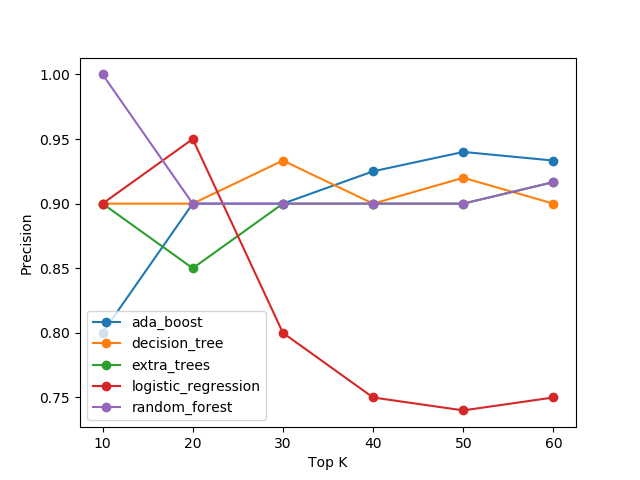
\includegraphics[scale=0.6]{plots/fakenewsexp1/precisionstopK.png}
% \caption{Precison at Top K instances that have the highest risk scores}
% \end{figure}
% the precision scores for some models decrease for higher K, some increase and some remain constant.

% \subsubsection{Recall at Top K}
% \begin{figure}[H]
% 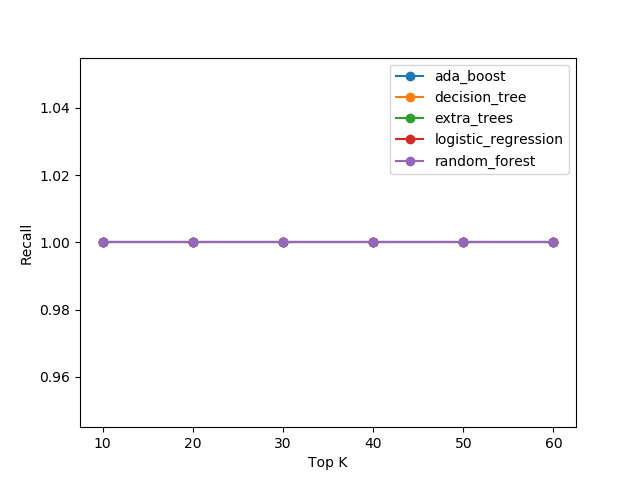
\includegraphics[scale=0.6]{plots/fakenewsexp1/recallstopK.png}
% \caption{Recall at Top K instances that have the highest risk scores}
% \end{figure}
% This plot is not good. Something is a bit off as the recall \textbf{remains at 1 }? Or perhaps all models are predicting only 1 class and not predicting for the other class. This is bad though. We must dig up the \textbf{contingency matrices} of the predictions of these models in the 2019 report


% \subsubsection{Jaccard Similarity at Top K}
% \begin{figure}[H]
% 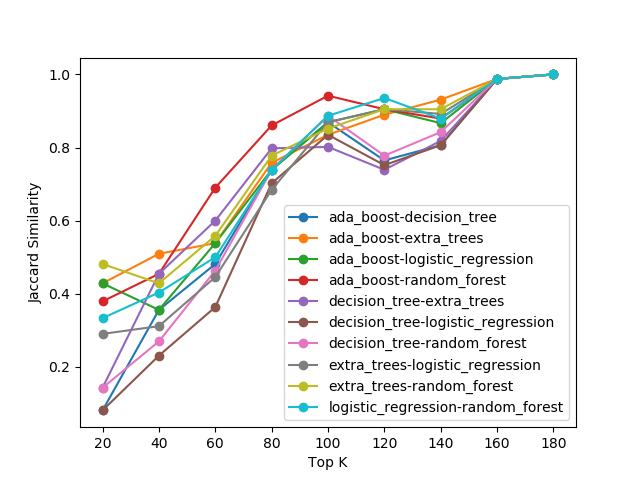
\includegraphics[scale=0.6]{plots/fakenewsexp1/jaccardtopK.png}
% \caption{Jaccard Similarity at Top K instances that have the highest risk scores}
% \end{figure}
% Some light in this plot. For any given K, the algorithms return the set of K news that are likely to be fake based on the risk scores. Good algorithms must return the same set of K instances that are likely to be fake.
% \noindent We realize that as the number of instances K increases, the similarity between all model pairs increase, with the highest similarity is between the Logistic Regression and the Random Forest models.

% \subsubsection{ROC Curves}
% \begin{figure}[H]
% 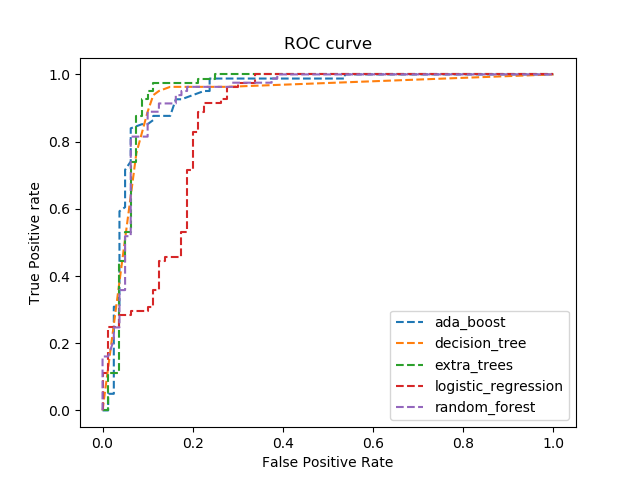
\includegraphics[scale=0.6]{plots/fakenewsexp1/roccurves.png}
% \caption{ROC Curves of predictions}
% \end{figure}
% The area under the curves for our models are good.

% \subsection{FP-Growth}
% In the figure below we show the frequent patterns that were extracted from the fake news data (FA-KES - Experiment 1) using FP Growth technique. Each \textbf{line} below represents a frequent pattern.
% \begin{figure}[H]
% \centering
% \includegraphics[scale=0.3]{plots/fakenewsexp1/fps.png}
% \end{figure}

% \textcolor{blue}{I did the probability of \textbf{mistake} per frequent pattern per model -- but I will leave it till the meeting to talk about it}



\end{document}